\documentclass{article}
\usepackage[utf8]{inputenc}
\usepackage{graphicx}
\usepackage{float}

\graphicspath{ {./images/} }

\title{\protect\parbox{\textwidth}{\protect\centering CS 300\\ Data Structures\\ Homework 5}}
%%\title{CS 300\newline Data Structures}
\author{Berkay Ersever}
\date{December 2018}

\usepackage{graphicx}
\usepackage{enumitem}

\begin{document}

\maketitle

\begin{figure}[H]
\centering
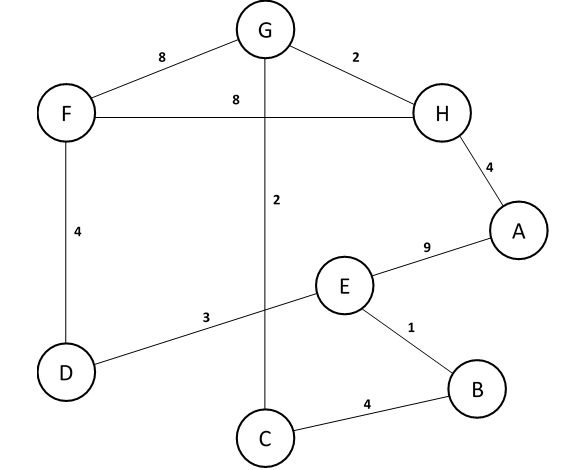
\includegraphics[scale=0.8]{figure-1}
\caption{An undirected weighted graph}
\end{figure}


\begin{enumerate}[leftmargin=\labelsep]
  \item[1.] Starting from G, trace the operations of the Dijkstra's weighted shortest path algorithm on the graph given in Figure 1.
\end{enumerate}

\begin{figure}[H]
\centering
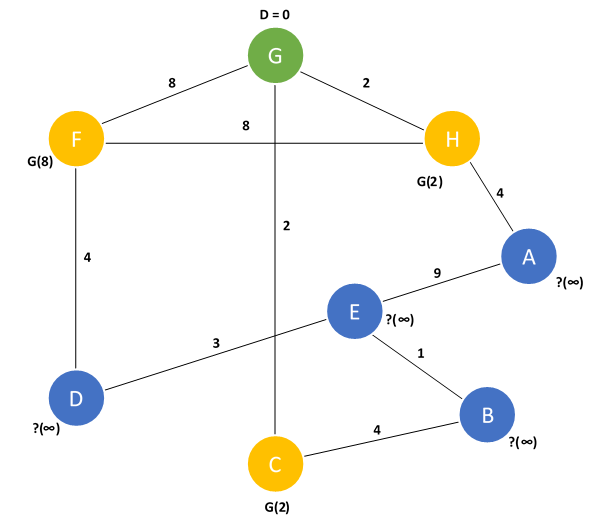
\includegraphics[scale=0.6]{images/Q1/01.png}
\end{figure}

\begin{figure}[H]
\centering
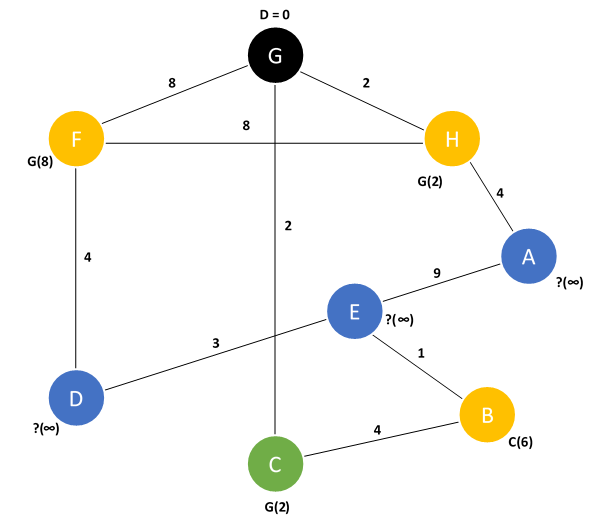
\includegraphics[scale=0.6]{images/Q1/02.png}
\end{figure}

\begin{figure}[H]
\centering
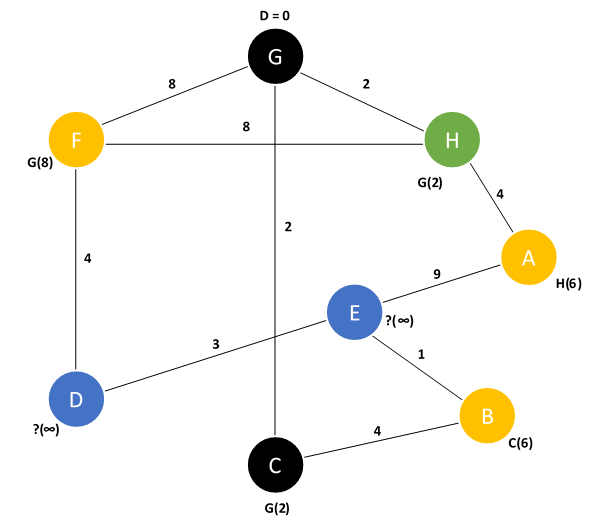
\includegraphics[scale=0.6]{images/Q1/03.png}
\end{figure}

\begin{figure}[H]
\centering
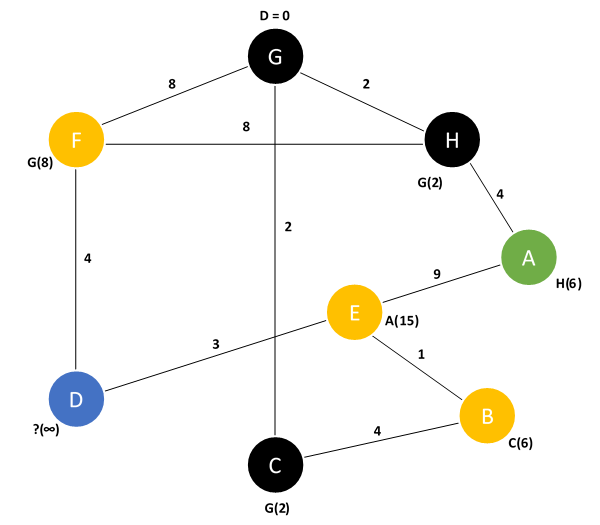
\includegraphics[scale=0.6]{images/Q1/04.png}
\end{figure}

\begin{figure}[H]
\centering
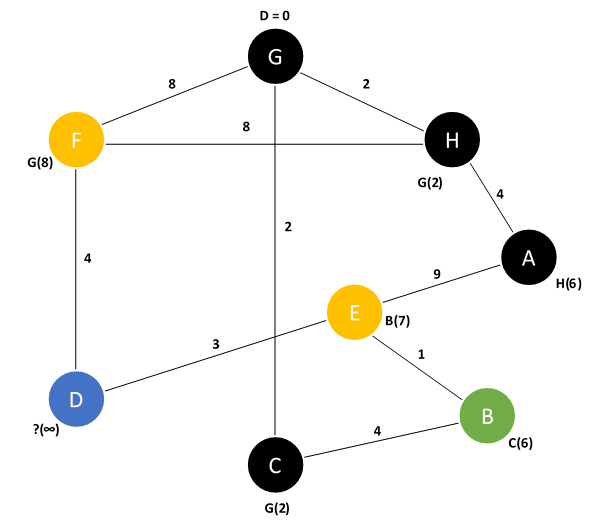
\includegraphics[scale=0.6]{images/Q1/05.png}
\end{figure}

\begin{figure}[H]
\centering
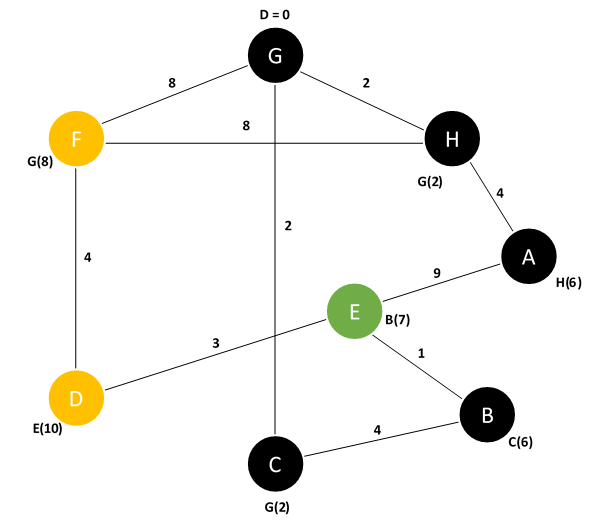
\includegraphics[scale=0.6]{images/Q1/06.png}
\end{figure}

\begin{figure}[H]
\centering
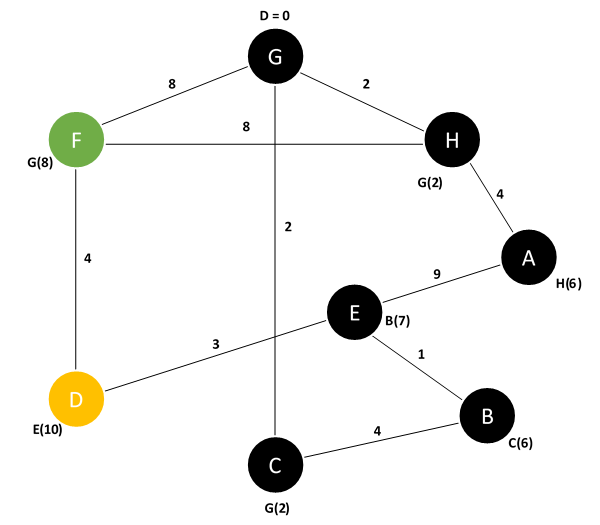
\includegraphics[scale=0.6]{images/Q1/07.png}
\end{figure}

\begin{figure}[H]
\centering
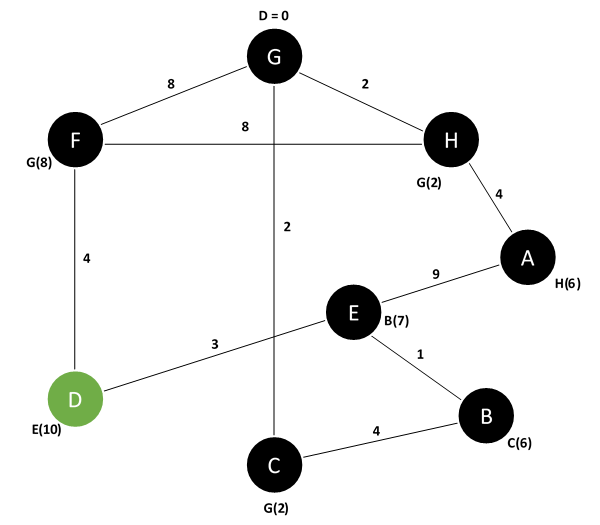
\includegraphics[scale=0.6]{images/Q1/08.png}
\end{figure}

\begin{figure}[H]
\centering
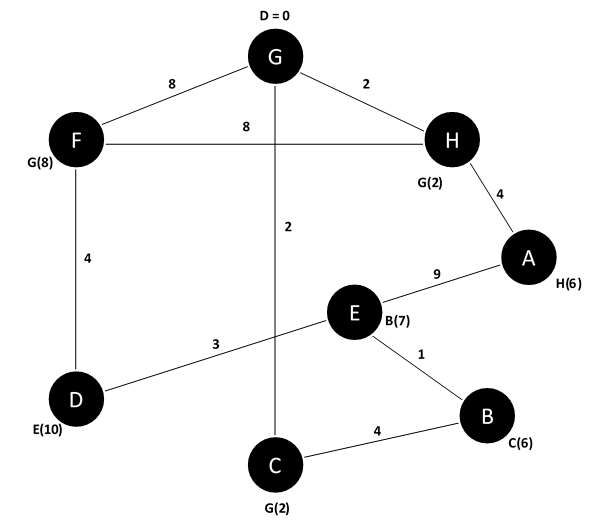
\includegraphics[scale=0.6]{images/Q1/09.png}
\end{figure}

\begin{enumerate}[leftmargin=\labelsep]
  \item[2.] Starting from G, trace the operations of the Prim's minimum spanning tree algorithm on the graph given in Figure 1.
\end{enumerate}

\begin{figure}[H]
\centering
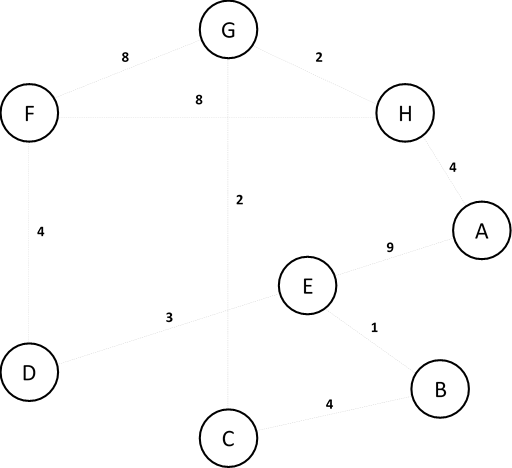
\includegraphics[scale=0.6]{images/Q2/01.png}
\end{figure}

\begin{figure}[H]
\centering
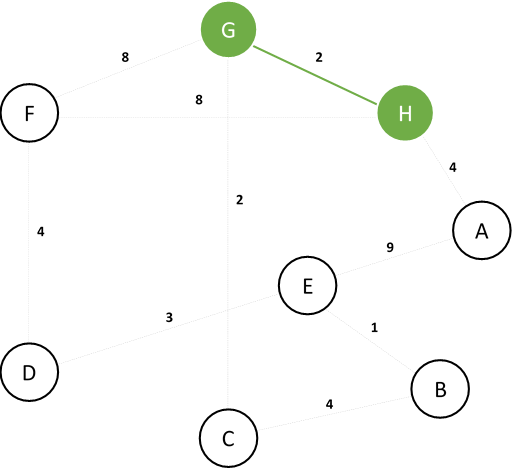
\includegraphics[scale=0.6]{images/Q2/02.png}
\end{figure}

\begin{figure}[H]
\centering
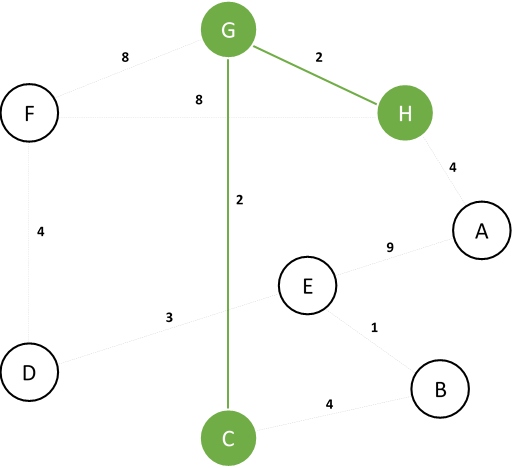
\includegraphics[scale=0.6]{images/Q2/03.png}
\end{figure}

\begin{figure}[H]
\centering
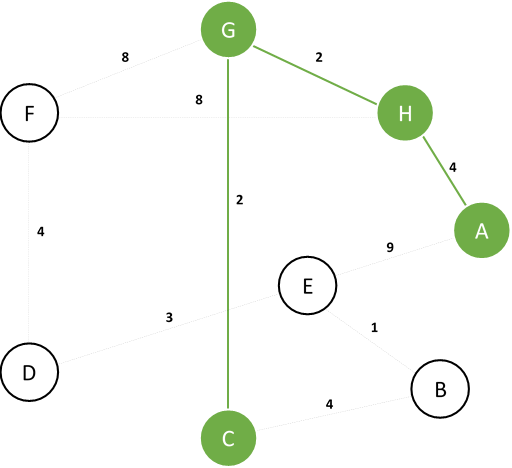
\includegraphics[scale=0.6]{images/Q2/04.png}
\end{figure}

\begin{figure}[H]
\centering
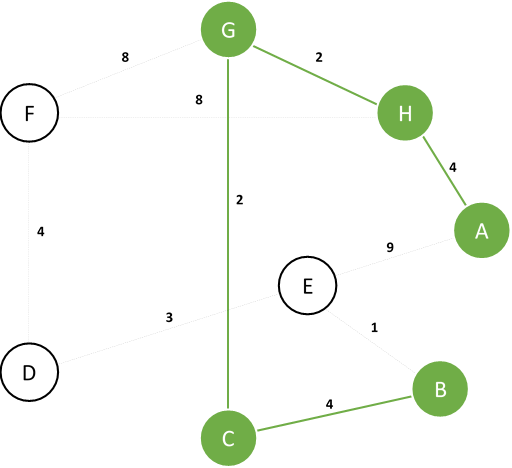
\includegraphics[scale=0.6]{images/Q2/05.png}
\end{figure}

\begin{figure}[H]
\centering
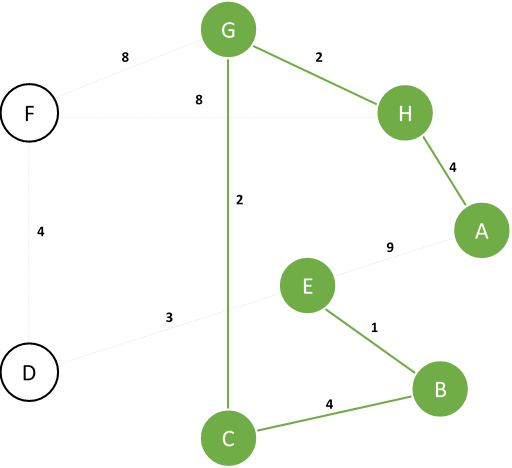
\includegraphics[scale=0.6]{images/Q2/06.png}
\end{figure}

\begin{figure}[H]
\centering
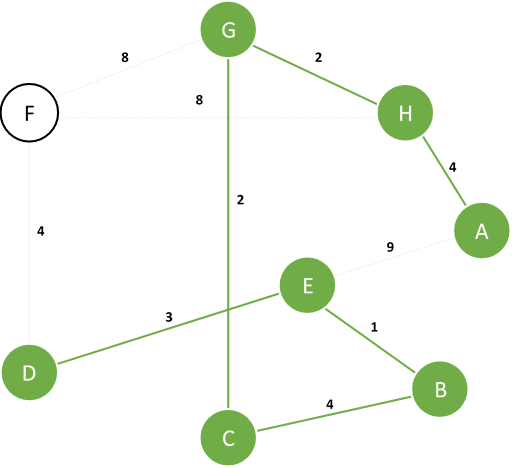
\includegraphics[scale=0.6]{images/Q2/07.png}
\end{figure}

\begin{figure}[H]
\centering
\includegraphics[scale=0.6]{images/Q2/08.png}
\end{figure}

\begin{enumerate}[leftmargin=\labelsep]
  \item[3.] Trace the operations of Kruskal's minimum spanning tree algorithm on the graph given in Figure 1.
\end{enumerate}

\begin{figure}[H]
\centering
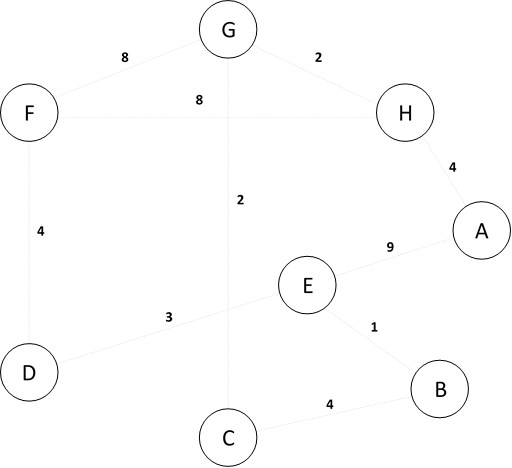
\includegraphics[scale=0.6]{images/Q3/01.png}
\end{figure}

\begin{figure}[H]
\centering
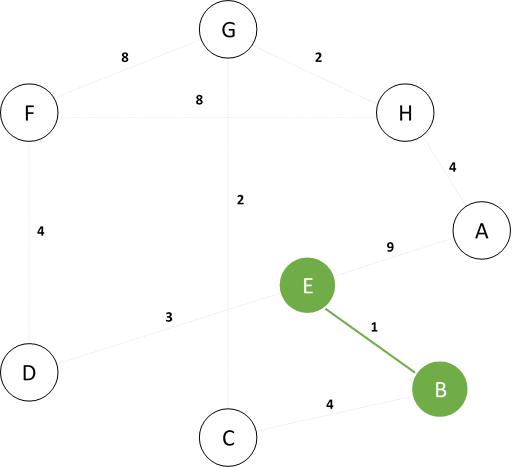
\includegraphics[scale=0.6]{images/Q3/02.png}
\end{figure}

\begin{figure}[H]
\centering
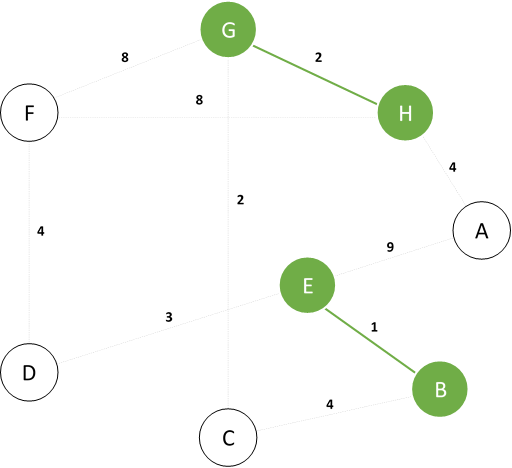
\includegraphics[scale=0.6]{images/Q3/03.png}
\end{figure}

\begin{figure}[H]
\centering
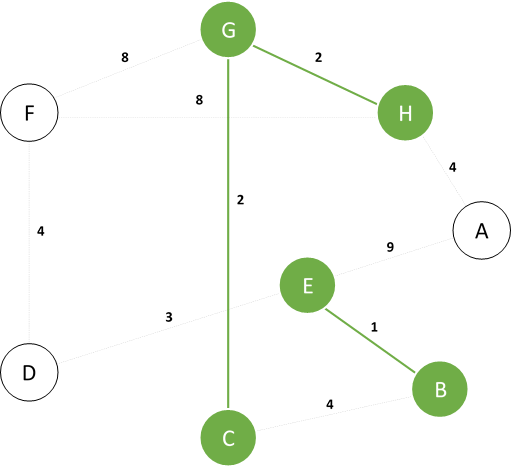
\includegraphics[scale=0.6]{images/Q3/04.png}
\end{figure}

\begin{figure}[H]
\centering
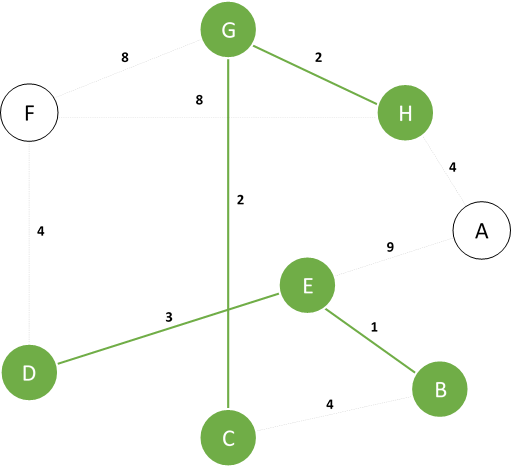
\includegraphics[scale=0.6]{images/Q3/05.png}
\end{figure}

\begin{figure}[H]
\centering
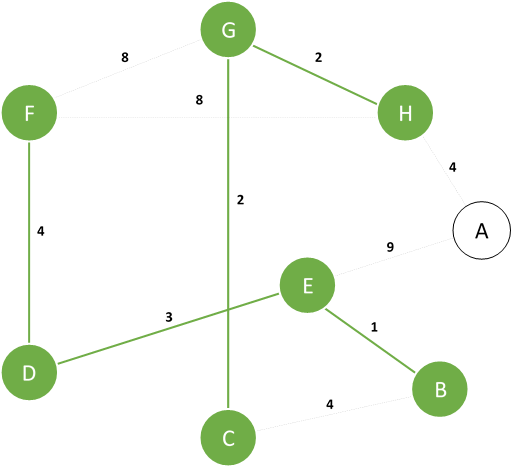
\includegraphics[scale=0.6]{images/Q3/06.png}
\end{figure}

\begin{figure}[H]
\centering
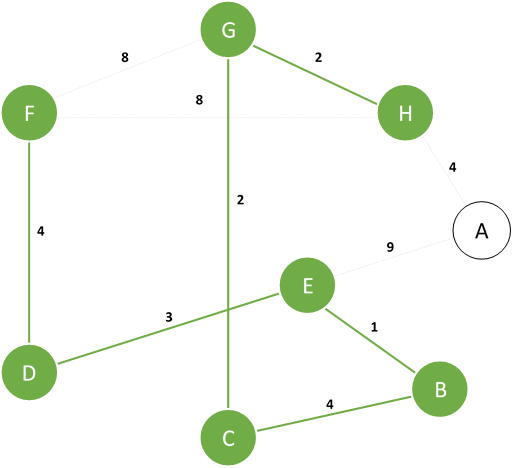
\includegraphics[scale=0.6]{images/Q3/07.png}
\end{figure}

\begin{figure}[H]
\centering
\includegraphics[scale=0.6]{images/Q3/08.png}
\end{figure}

\begin{figure}[H]
\centering
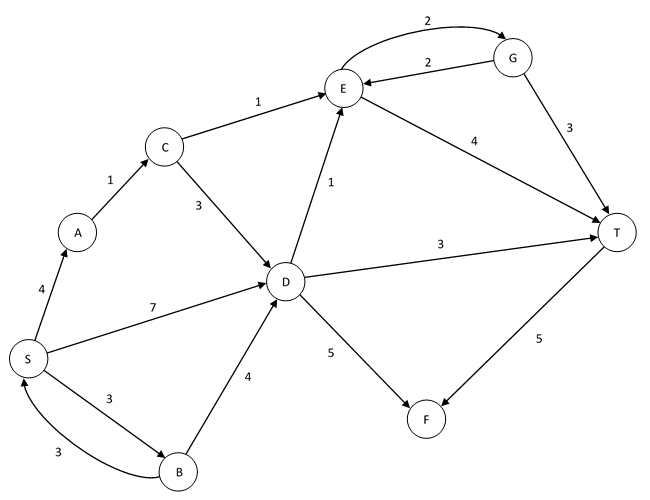
\includegraphics[scale=0.8]{figure-2}
\caption{A directed weighted graph}
\end{figure}

\begin{enumerate}[leftmargin=\labelsep]
  \item[4.] Starting from S, trace the operations of breadth-first traversal on the graph given in Figure 2.
\end{enumerate}

\begin{figure}[H]
\centering
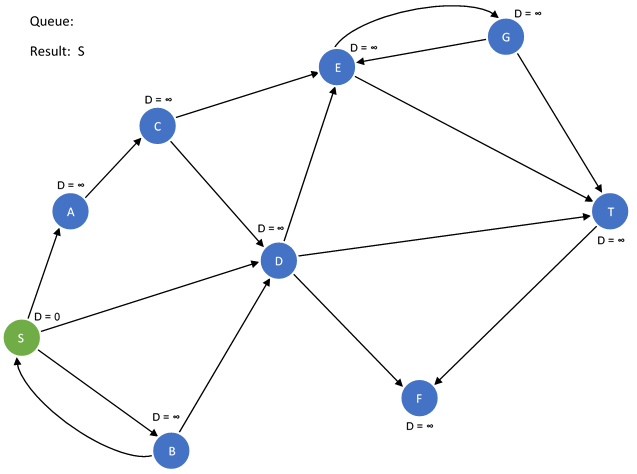
\includegraphics[scale=0.6]{images/Q4/01.png}
\end{figure}

\begin{figure}[H]
\centering
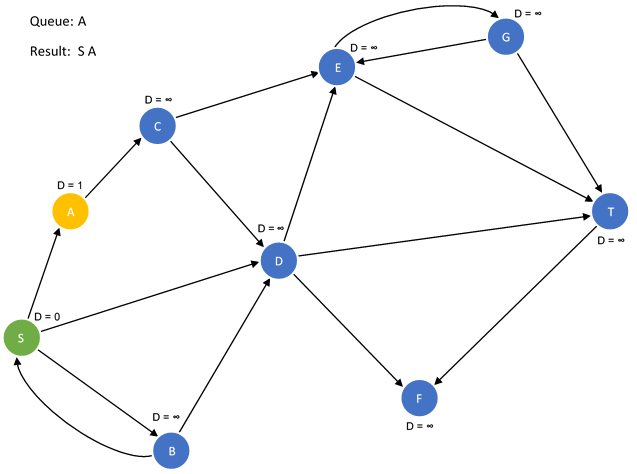
\includegraphics[scale=0.6]{images/Q4/02.png}
\end{figure}

\begin{figure}[H]
\centering
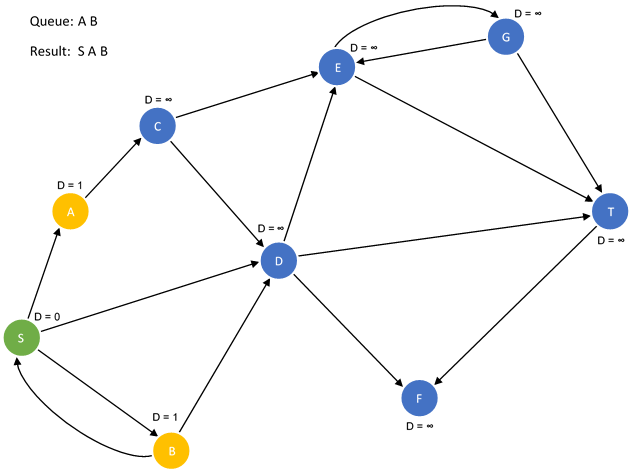
\includegraphics[scale=0.6]{images/Q4/03.png}
\end{figure}

\begin{figure}[H]
\centering
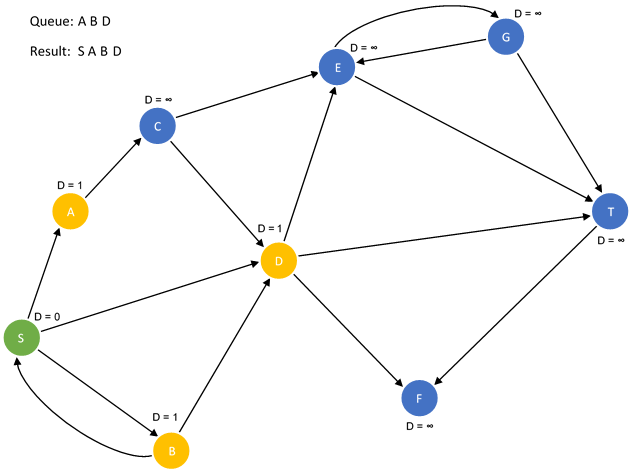
\includegraphics[scale=0.6]{images/Q4/04.png}
\end{figure}

\begin{figure}[H]
\centering
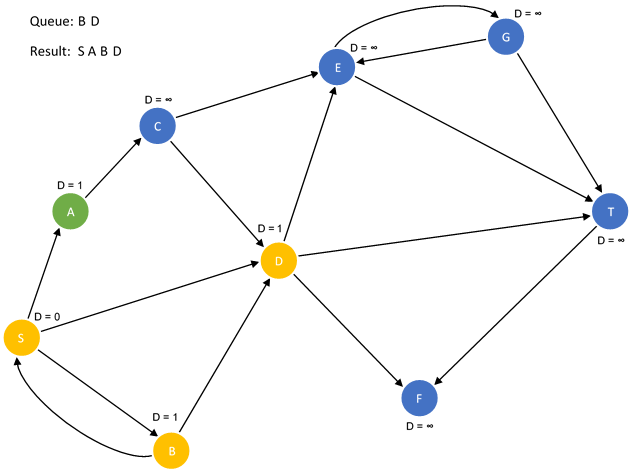
\includegraphics[scale=0.6]{images/Q4/05.png}
\end{figure}

\begin{figure}[H]
\centering
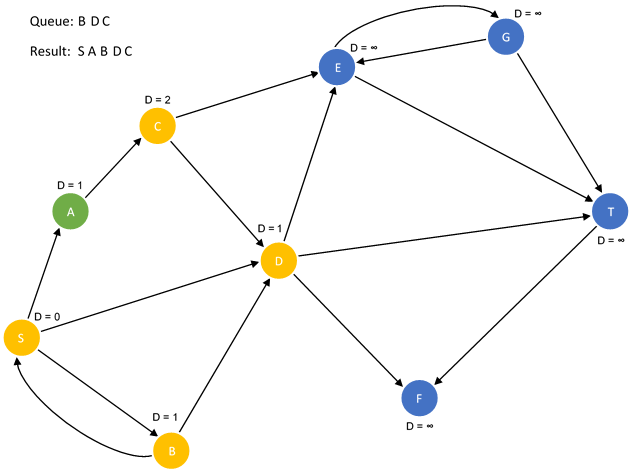
\includegraphics[scale=0.6]{images/Q4/06.png}
\end{figure}

\begin{figure}[H]
\centering
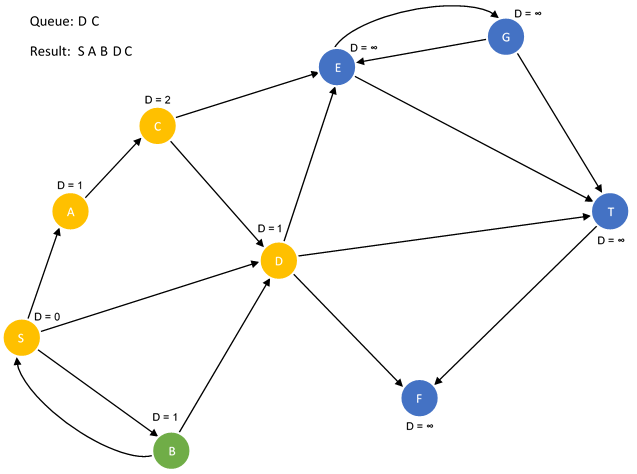
\includegraphics[scale=0.6]{images/Q4/07.png}
\end{figure}

\begin{figure}[H]
\centering
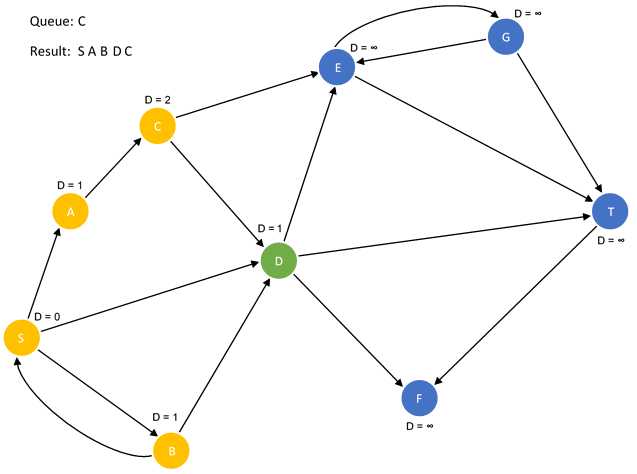
\includegraphics[scale=0.6]{images/Q4/08.png}
\end{figure}

\begin{figure}[H]
\centering
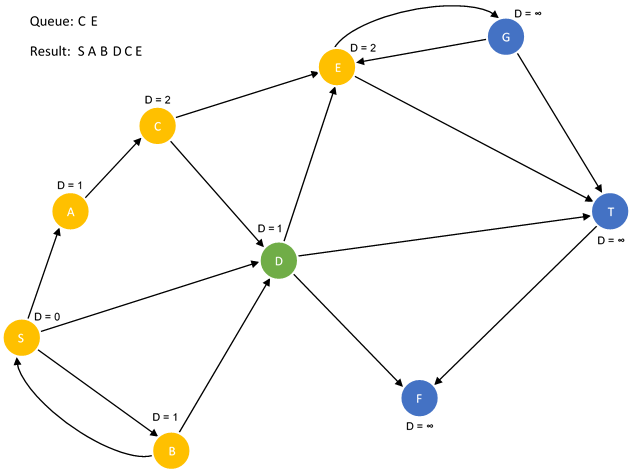
\includegraphics[scale=0.6]{images/Q4/09.png}
\end{figure}

\begin{figure}[H]
\centering
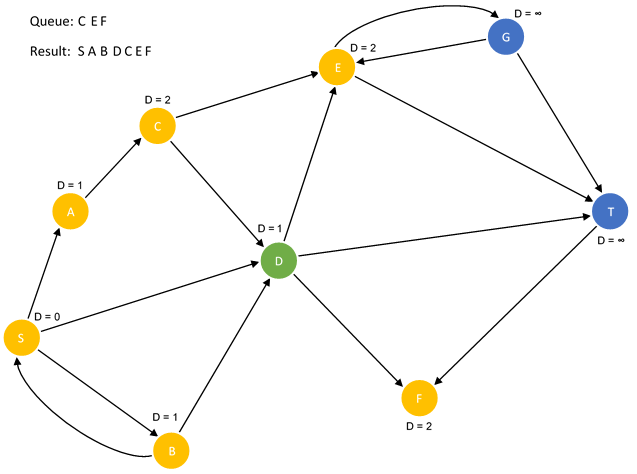
\includegraphics[scale=0.6]{images/Q4/10.png}
\end{figure}

\begin{figure}[H]
\centering
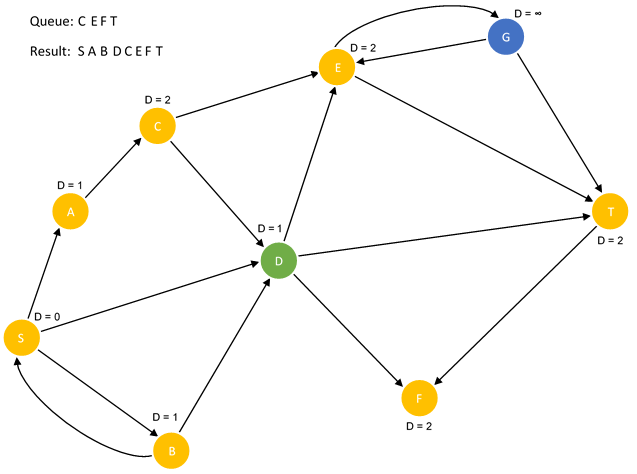
\includegraphics[scale=0.6]{images/Q4/11.png}
\end{figure}

\begin{figure}[H]
\centering
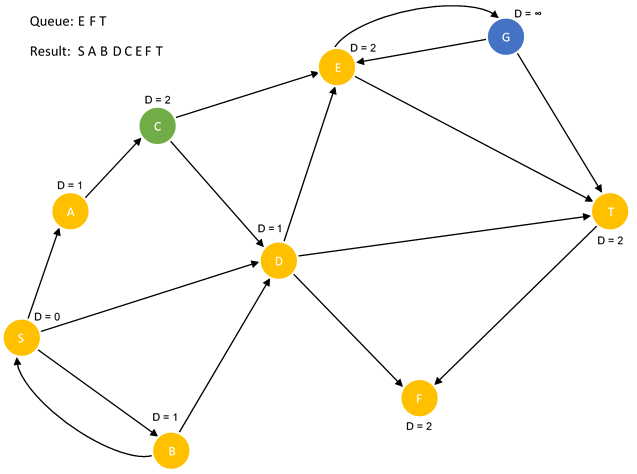
\includegraphics[scale=0.6]{images/Q4/12.png}
\end{figure}

\begin{figure}[H]
\centering
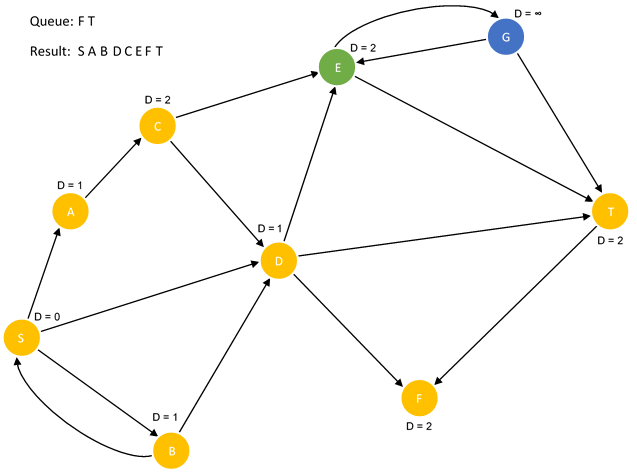
\includegraphics[scale=0.6]{images/Q4/13.png}
\end{figure}

\begin{figure}[H]
\centering
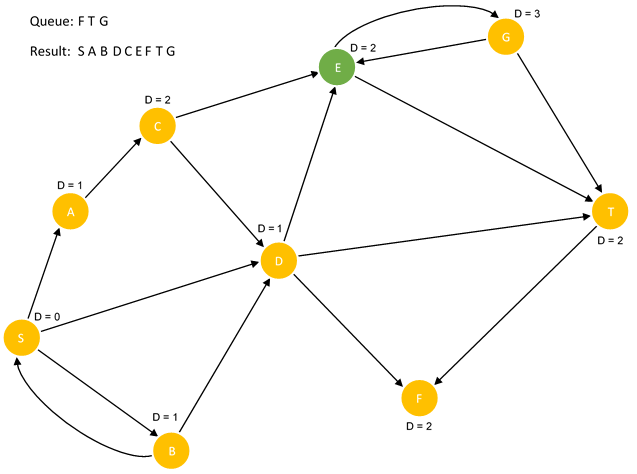
\includegraphics[scale=0.6]{images/Q4/14.png}
\end{figure}

\begin{figure}[H]
\centering
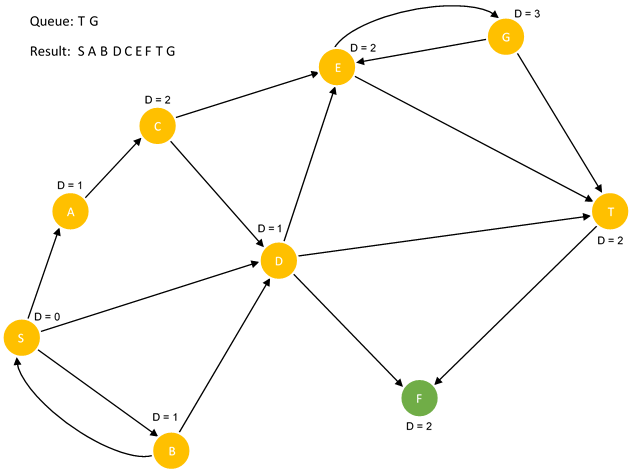
\includegraphics[scale=0.6]{images/Q4/15.png}
\end{figure}

\begin{figure}[H]
\centering
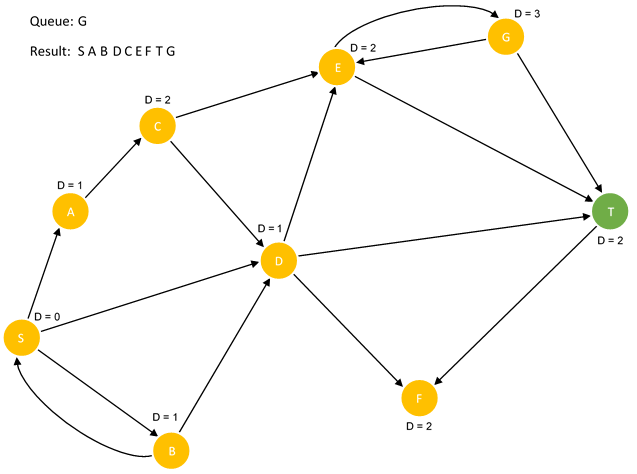
\includegraphics[scale=0.6]{images/Q4/16.png}
\end{figure}

\begin{figure}[H]
\centering
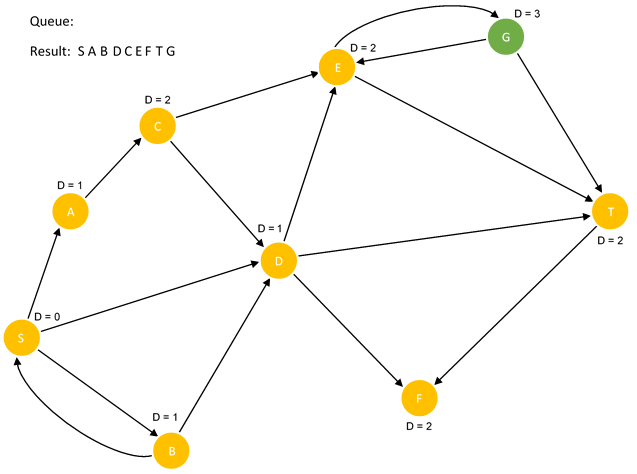
\includegraphics[scale=0.6]{images/Q4/17.png}
\end{figure}

\begin{figure}[H]
\centering
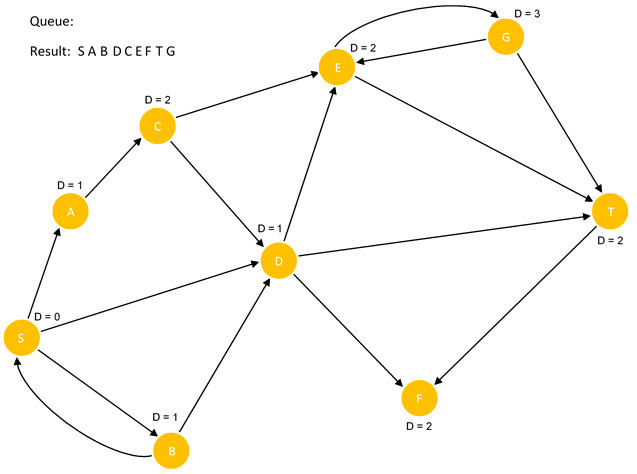
\includegraphics[scale=0.6]{images/Q4/18.png}
\end{figure}

\begin{center}
\textit{\\S - A - B - D - C - E - F - T - G\\}
\end{center}
\newpage

\begin{enumerate}[leftmargin=\labelsep]
  \item[5.] Given Figure 2 and starting from S,
  \begin{enumerate}[leftmargin=\labelsep]
    \item[a)] Trace the operations of depth-first traversal.
  \end{enumerate}

\begin{figure}[H]
\centering
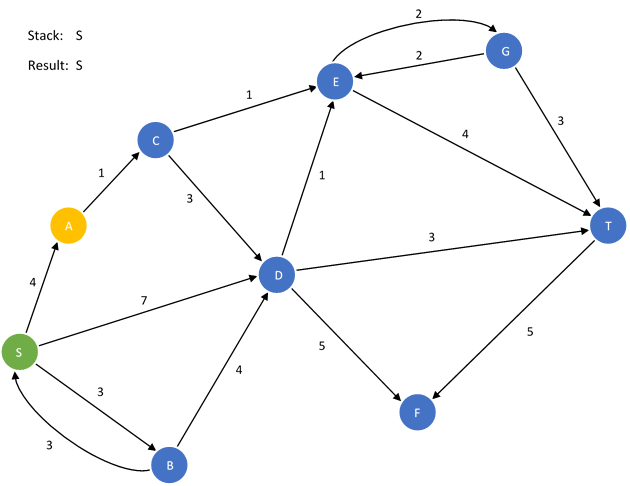
\includegraphics[scale=0.6]{images/Q5/a/01.png}
\end{figure}

\begin{figure}[H]
\centering
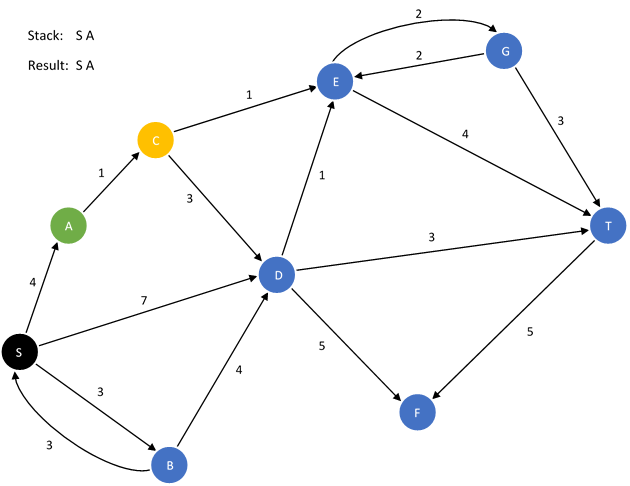
\includegraphics[scale=0.6]{images/Q5/a/02.png}
\end{figure}

\begin{figure}[H]
\centering
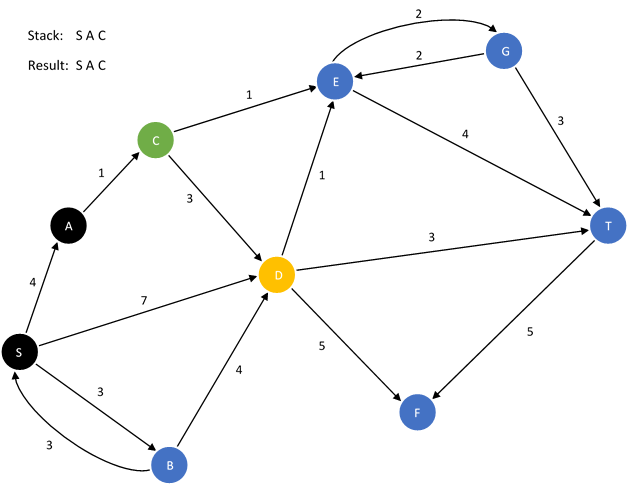
\includegraphics[scale=0.6]{images/Q5/a/03.png}
\end{figure}

\begin{figure}[H]
\centering
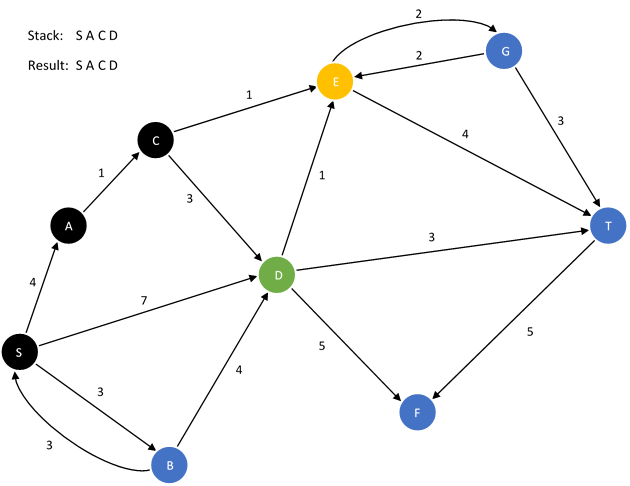
\includegraphics[scale=0.6]{images/Q5/a/04.png}
\end{figure}

\begin{figure}[H]
\centering
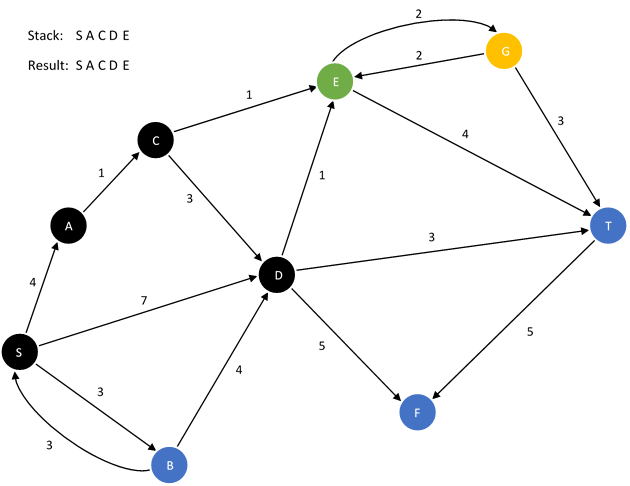
\includegraphics[scale=0.6]{images/Q5/a/05.png}
\end{figure}

\begin{figure}[H]
\centering
\includegraphics[scale=0.6]{images/Q5/a/06.png}
\end{figure}

\begin{figure}[H]
\centering
\includegraphics[scale=0.6]{images/Q5/a/07.png}
\end{figure}

\begin{figure}[H]
\centering
\includegraphics[scale=0.6]{images/Q5/a/08.png}
\end{figure}

\begin{figure}[H]
\centering
\includegraphics[scale=0.6]{images/Q5/a/09.png}
\end{figure}

\begin{figure}[H]
\centering
\includegraphics[scale=0.6]{images/Q5/a/10.png}
\end{figure}

\begin{figure}[H]
\centering
\includegraphics[scale=0.6]{images/Q5/a/11.png}
\end{figure}

\begin{figure}[H]
\centering
\includegraphics[scale=0.6]{images/Q5/a/12.png}
\end{figure}

\begin{figure}[H]
\centering
\includegraphics[scale=0.6]{images/Q5/a/13.png}
\end{figure}

\begin{figure}[H]
\centering
\includegraphics[scale=0.6]{images/Q5/a/14.png}
\end{figure}

\begin{figure}[H]
\centering
\includegraphics[scale=0.6]{images/Q5/a/15.png}
\end{figure}

\begin{figure}[H]
\centering
\includegraphics[scale=0.6]{images/Q5/a/16.png}
\end{figure}

\begin{figure}[H]
\centering
\includegraphics[scale=0.6]{images/Q5/a/17.png}
\end{figure}

\begin{figure}[H]
\centering
\includegraphics[scale=0.6]{images/Q5/a/18.png}
\end{figure}

\newpage
  \begin{enumerate}[leftmargin=\labelsep]
    \item[b)] Give the post-order numbers for all the nodes.
  \end{enumerate}

\begin{center}
\begin{tabular}{ |c|c|c|c|c|c|c|c|c|c| } 
 \hline
  \textbf{Nodes} & F & T & G & E & D & C & A & B & S \\ 
 \hline
  \textbf{Post-Order} & 1 & 2 & 3 & 4 & 5 & 6 & 7 & 8 & 9 \\ 
 \hline
\end{tabular}
\end{center}

  \begin{enumerate}[leftmargin=\labelsep]
    \item[c)] Give the pre-order numbers for all the nodes.
  \end{enumerate}

\begin{center}
\begin{tabular}{ |c|c|c|c|c|c|c|c|c|c| } 
 \hline
  \textbf{Nodes} & S & A & C & D & E & G & T & F & B \\ 
 \hline
  \textbf{Pre-Order} & 1 & 2 & 3 & 4 & 5 & 6 & 7 & 8 & 9 \\ 
 \hline
\end{tabular}
\end{center}

  \begin{enumerate}[leftmargin=\labelsep]
    \item[d)] List the tree arcs, cross arcs, forward arcs and backward arcs.
  \end{enumerate}

\begin{center}
\begin{tabular}{ |c|c|c|c| } 
 \hline
  \textbf{Tree Arcs} & \textbf{Cross Arcs} & \textbf{Forward Arcs} & \textbf{Backward Arcs} \\ 
 \hline
  S$\rightarrow$B & B$\rightarrow$D & S$\rightarrow$D & G$\rightarrow$E \\
 \hline
  S$\rightarrow$A &  & C$\rightarrow$E & B$\rightarrow$S \\
 \hline
  A$\rightarrow$C &  & D$\rightarrow$T &  \\
 \hline
  C$\rightarrow$D &  & D$\rightarrow$F &  \\
 \hline
  D$\rightarrow$E &  & E$\rightarrow$T &  \\
 \hline
  E$\rightarrow$G &  &  &  \\
 \hline
  G$\rightarrow$T &  &  &  \\
 \hline
  T$\rightarrow$F &  &  &  \\
 \hline
\end{tabular}
\newline
\newline
\newline
\end{center}
\end{enumerate}

\begin{figure}[H]
\centering
\includegraphics[scale=0.8]{figure-3.png}
\caption{An example DAG}
\end{figure}

\newpage

\begin{enumerate}[leftmargin=\labelsep]
  \item[6.] Find a topological ordering of the graph given in Figure 3.
  \newline
\end{enumerate}

\begin{figure}[H]
\centering
\includegraphics[scale=0.6]{images/Q6/01.png}
\end{figure}

\begin{figure}[H]
\centering
\includegraphics[scale=0.6]{images/Q6/02.png}
\end{figure}

\begin{figure}[H]
\centering
\includegraphics[scale=0.6]{images/Q6/03.png}
\end{figure}

\begin{figure}[H]
\centering
\includegraphics[scale=0.6]{images/Q6/04.png}
\end{figure}

\begin{figure}[H]
\centering
\includegraphics[scale=0.6]{images/Q6/05.png}
\end{figure}

\begin{figure}[H]
\centering
\includegraphics[scale=0.6]{images/Q6/06.png}
\end{figure}

\begin{figure}[H]
\centering
\includegraphics[scale=0.6]{images/Q6/07.png}
\end{figure}

\begin{center}
\textit{\\\textbf{Topological ordering of the graph: A-B-C-G-D-E-F\\}}
\end{center}

\end{document}
